\section{The Components of the Jeliot~3 System}
\label{sec:The_Components_of_the_Jeliot_3_System}




\subsection{Visualization Engine}
\label{sec:Visualization_Engine}




\subsection{DynamicJava}
\label{sec:DynamicJava}

Dynamic Java is a Java source code interpreter written in Java. This application is open source and can be freely obtained . At the moment, DynamicJava is almost fully compliant with Java specifications and supports multi-threading. Due to the lack of documentation (nothing is provided except an API documentation done by JavaDoc) it was necessary to take a look to the source code of the software to understand its behaviour. There we obtained the following relevant information:

DynamicJava consists of 7 different packages, where only five of them actually perform the interpretation: classfile, classinfo, interpreter, parser and tree. The other two (util and gui) are used to help the debugging of DynamicJava and to provide a nicer user interface to the interpreter. For example, the displayVisitor, included in the util package, provides a nice output from the syntax tree.

\begin{itemize}
\item {\bf{Classfile}} contains all the classes for creating general purpose bytecode classes. The most important class is ClassFile which is the heart of the class creation process.
\item {\bf{Classinfo}} contains all the classes and interfaces for using reflection on Java or interpreted classes. This package is used during the compilation of the classes.
\item {\bf{Interpreter}} contains the classes for interpreting Java language statements. This is the most important package. It contains the most important visitors that will be explained later.
\item {\bf{Parser}} provides the classes that compose the default parser for the language. The parser itself is represented by the class Parser. All the Java files were generated by JavaCC 1.0. It creates the nodes of the tree to be traversed later by the interpreter visitors.
\item {\bf{Tree}} provides classes and interfaces for producing an abstract syntax tree. This package does not depend of any non standard java package.
\end{itemize}

The created tree consists of nodes, the main data structure used in DynamicJava. All nodes have common properties, the segment of source code where that node refers. Subclasses of this node are defined to address the unique properties of each different Java (e.g. staments and constructions). For example a node for any binary expression will also consist of the properties LEFT\_EXRESSION and RIGHT\_EXPRESSION.

The following Figure~\ref{fig:djava_structure} explains the main relationships between the packages, the visitors and the main data flow.

\begin{figure}[!htb]
\begin{center}
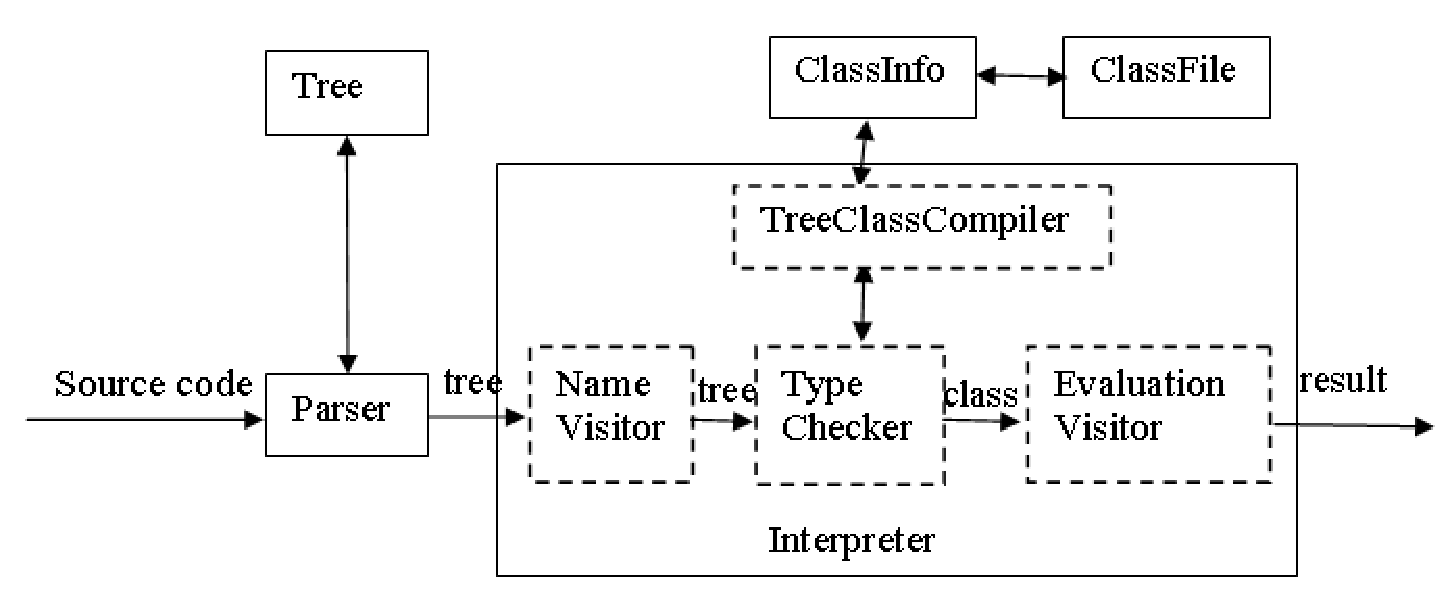
\includegraphics[height=6cm]{djava_structure.eps}
\caption{The package structure and dependencies between packages in DynamicJava.}
\label{fig:djava_structure}
\end{center}
\end{figure}

As we can see in the image DynamicJava carries the source code through 3 visitors: NameVisitor, TypeChecker and, finally, EvaluationVisitor. We also see how EvaluationVisitor will receive a class from TypeChecker, the reason of this behaviour will be explained in the next paragraphs and in the section dedicated to the Concurrent Interpreter

\subsection{NameVisitor}

This tree visitor resolves the ambiguity in identifiers in a syntax tree. As declared, this visitor traverses the tree trying to find out syntactical ambiguities.

\subsection{TypeChecker}

This tree visitor checks the typing rules and loads the classes, fields and methods. This TypeChecker class is not only worried about typing rules. When visiting a class declaration, it invokes TreeCompiler, which compile the class into Java bytecode. However this compiling process alters the class and the formed byte code does not match the original source code of the class.

\subsection{EvaluationVisitor}

This tree visitor evaluates each node of a syntax tree. This visitor is the one that performs the evaluation and execution of the program. It usually starts by invoking the main method of the compiled class. We can easily observe how it traverses the syntax tree and modifies DynamicJava structures to store information and thus we can interfere with its normal interpretation to extract the information it produces while interpreting the source code.
